% !TeX root = ../../libro.tex
% !TeX encoding = utf8

A continuación se enuncian resultados de la Teoría de Morse, principalmente utilizados para la demostración de los Hechos.

\begin{teorema}
	Sea $S$ superficie y $f: S \rightarrow \R$ función de Morse. Tomamos $a < b$ valores regulares tal que $W(a,b)$ no contiene ningún punto crítico de $f$. Entonces:
	\begin{itemize}
		\item $M(b)$ es difeomorfo a $M(a)$.
		\item $V(b)$ es difeomorfo a $V(a)$.
		\item $W(a,b)$ es difeomorfo a $V(a) \times [a,b]$, o de forma equivalente, cada componente conexa de $W(a,b)$ es difeomorfa a un anillo de $\R^2$.
	\end{itemize}
\end{teorema}

\begin{proof}
	Se demuestra en el artículo ``Clasification of Surface via Morse Theory'' \cite{MorseTh1}, el teorema 8.
\end{proof}

\begin{teorema}
	Sea $S$ superficie y $f: S \rightarrow \R$ función de Morse. Sea $p$ un punto crítico y $a < b$ valores regulares tal que $W(a,b)$ no contiene ningún punto crítico de $f$ aparte de $p$. Entonces:
	\begin{itemize}
		\item Si el índice de $p$ es $0$ o $2$, $M(b)$ es difeomorfo a la unión disjunta de $M(a)$ con un disco $D$, es decir, $W(a,b)$ es difeomorfo a un disco $D$.
		\item Si el índice de $p$ es $1$, $M(b)$ es difeomorfo a $M(a)$ junto con un rectángulo pegado  en dos segmentos disjnutos de $V(a)$, que se puede ver como unos ``pantalones'' si el pegado se realiza de acuerdo a la orientación, o unos ``pantalones cruzados'' en caso contrario.
	\end{itemize}
\end{teorema}

\begin{figure}[h]
  	\centering
  	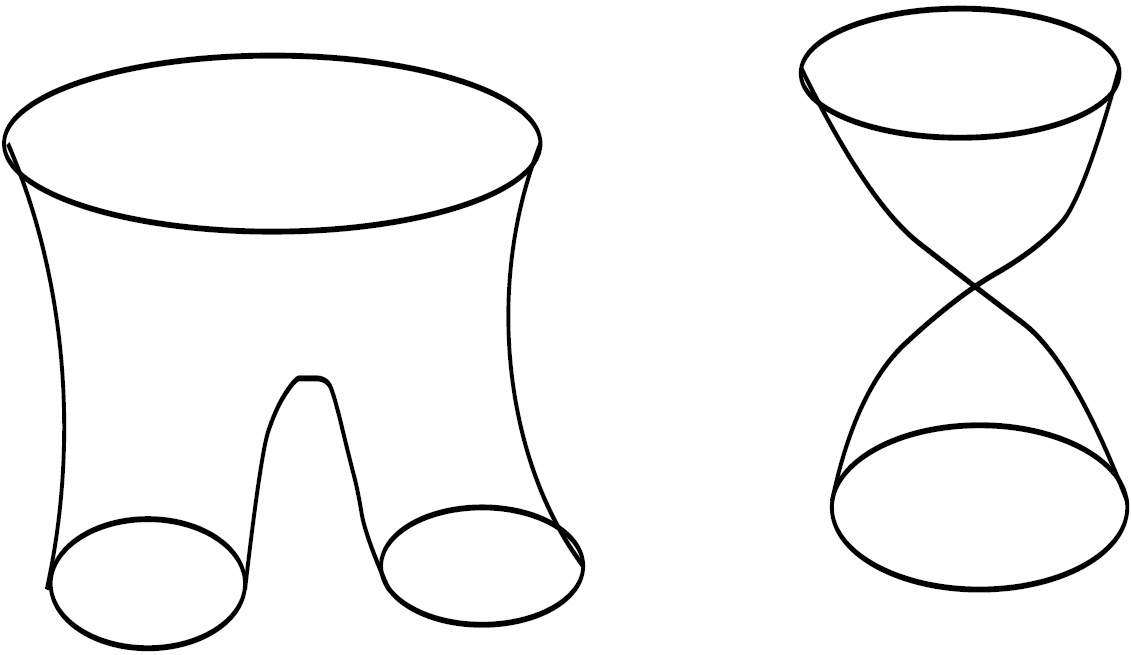
\includegraphics[width=0.4\textwidth]{pantalones}
  	\caption{Pantalones normales y cruzados}
  	\label{fig:pantalones}
\end{figure}

\begin{proof}
	El primer punto se demuestra en el artículo ``Clasification of Surface via Morse Theory'' \cite{MorseTh1}, el teorema 13. El punto siguiente se demuestra en el mismo artículo, el teorema 16.
\end{proof}

\endinput
%------------------------------------------------------------------------------------
% FIN DEL CAPÍTULO. 
%------------------------------------------------------------------------------------
